%% LyX 2.2.2 created this file.  For more info, see http://www.lyx.org/.
%% Do not edit unless you really know what you are doing.
\documentclass[11pt,english]{beamer}
\usepackage{enumerate}
% \usepackage{enumitem} % para cambiar los bullets en el enumerate
\usepackage{mathptmx}
\usepackage[T1]{fontenc}
\usepackage[utf8]{inputenc}
\setlength{\parskip}{\smallskipamount}
\setlength{\parindent}{0pt}
\usepackage{url}
\usepackage[authoryear]{natbib}
\usefonttheme[onlymath]{serif} % para las fuentes de las ecuaciones
\makeatletter
\usepackage{amsmath,amssymb,amsthm}
\usepackage{graphicx}
\usepackage{xcolor} % para colorear textos con \textcolor o \color
\usepackage{hyperref}
\usepackage{times}
\usepackage{array}
\usepackage{multicol}
\usepackage{longtable}
\usepackage{float} % para usar comando [H] en tablas y gr\'aficas
\usepackage{xcolor}% para modificar el color de la presentacion y del texto
\usepackage{colortbl} % para tablas de Kable
\usepackage{booktabs} % Para toprule: To thicken table lines 
\usepackage[nogin]{Sweave} % elimina el tamaño por default de las figuras de sweave
\usepackage{natbib}
\bibliographystyle{agsm}
% \usepackage[inline]{enumitem} % para enumerar dentro de un paragrafo
\usepackage{rotating} % para rotar nombres de columnas

\usepackage{fancyvrb} % Ensure this line is in your preamble
\usepackage{graphicx}
\usepackage{subcaption}

\usepackage{listings} % esta y la siguiente para resolver el problema del FancyVerb 
\lstset{basicstyle=\ttfamily} % esta tambien para lo del FancyVerb 



%%%%%%%%%%%%%%%%%%%%%%%%%%%%%% LyX specific LaTeX commands.
\providecommand{\LyX}{L\kern-.1667em\lower.25em\hbox{Y}\kern-.125emX\@}

%%%%%%%%%%%%%%%%%%%%%%%%%%%%%% Textclass specific LaTeX commands.
 % this default might be overridden by plain title style
 \newcommand\makebeamertitle{\frame{\maketitle}}%
 % (ERT) argument for the TOC
 \AtBeginDocument{%
   \let\origtableofcontents=\tableofcontents
   \def\tableofcontents{\@ifnextchar[{\origtableofcontents}{\gobbletableofcontents}}
   \def\gobbletableofcontents#1{\origtableofcontents}
 }
\newcommand{\code}[1]{\texttt{#1}}

%%%%%%%%%%%%%%%%%%%%%%%%%%%%%% User specified LaTeX commands.
\usetheme{Warsaw}
% or ...

\setbeamercovered{transparent}
% or whatever (possibly just delete it)

\usepackage[T1]{fontenc}

\makeatother

\usepackage{babel}
\usepackage{listings}
\renewcommand{\lstlistingname}{\inputencoding{latin9}Listing}

\begin{document}
\Sconcordance{concordance:5_ACS.tex:5_ACS.Rnw:1 52 1 1 4 50 1 5 4 1 1 1 4 1 5 3 4 173 %
1 1 8 2 1 1 7 55 0 1 2 40 1 1 9 16 0 1 2 11 1 1 9 16 0 1 2 5 1 1 7 1 2 %
37 1 1 8 2 1 1 10 16 0 1 2 6 1 1 7 1 2 4 1 1 11 18 0 1 2 6 1 1 8 1 2 %
164 1 1 6 4 1 1 17 16 0 1 2 7 1 1 5 1 2 7 1 1 14 15 0 1 2 8 1 1 4 1 2 3 %
1 1 12 3 1 1 5 2 1 2 2 43 1}



\title{Análisis de Correspondencias Simples (ACS)}

\subtitle{Introducción}

\author{Jimmy A Corzo S\inst{1} \inst{2}}

\institute[Profesor Titular]{\inst{1}Profesor Titular\\
Departamento de Estadística\and \inst{2}Facultad de ciencias\\
Universidad Nacional de colombia}

\date[2023]{Métodos multivariados aplicados \LyX{} cap 3}

\makebeamertitle

%\pgfdeclareimage[height=0.5cm]{institution-logo}{institution-logo-filename}

%\logo{\pgfuseimage{institution-logo}}

\AtBeginSubsection[]{

  \frame<beamer>{ 

    \frametitle{Outline}   

    \tableofcontents[currentsection,currentsubsection] 

  }

}













%\beamerdefaultoverlayspecification{<+->}
\begin{frame}
\tableofcontents{}
\end{frame}

\section{Descripción del método}
\begin{frame}{Introducción}
EL ACS es un método de análisis de tablas de contingencia, cuyas celdas contienen las frecuencias de las opciones o modalidades de respuesta de variables cualitativas. 

Esto distingue considerablemente el ACS del ACP el cual requiere que las variables observadas están en escalas cuantitativas.

Las escalas de las variables cualitativas representan \textbf{códigos} asignados a las respuestas, los cuales pueden representar jerarquías como el estrato socioeconómicoo el nivel educativo, o simplemente distinguir entre objetos o entes como las ciudades, las universidades, los países, el estado civil, etc. 
\end{frame}

% _________________________________________
\begin{frame}{Escalas de medida de variables cualitativas}
\begin{itemize}
	\item \textbf{Nominal} donde los códigos corresponden a clasificaciones \textbf{no ordenadas} de objetos como máquinas, universidades, países, o a cualidades humanas como sexo, la raza, o clasificaciones sociales como el estado civil etc.
	
	\item \textbf{Ordinal o categórica}  cuyos códigos o categorías de respuesta indican \textbf{orden o jerarquía} el estrato o nivel socioeconómico, el nivel educativo, las posiciones que ocupan los competidores en una carrera, o las universidades en los rankings.
\end{itemize}

\end{frame}
% 
\begin{frame}
\begin{itemize}
	\item \textbf{Likert} que es una escala ordinal en la cual se codifican los grados de aprobación (desaprobación) de actitudes o situaciones, o los grados de acuerdo (desacuerdo) con actitudes o afirmaciones. Las modalidades más comunes son \textit{totalmente en desacuerdo}, \textit{en desacuerdo}, \textit{indiferente}, \textit{de acuerdo} y \textit{totalmente de acuerdo}; o la frecuencia con que se realiza una actividad o actitud en escalas como \textit{nunca}, \textit{casi nunca}, \textit{casi siempre}, \textit{siempre}.
	
	\item \textbf{Hedonista} que también es una escala categórica cuyos códigos ordenan los niveles de preferencia o de agrado con situaciones o estímulos. Algunas modalidades utilizadas son: me desagrada mucho, me desagrada, ni me agrada ni me desagrada, me agrada, me agrada mucho
\end{itemize}

\end{frame}
% 
\begin{frame}
Las \textbf{opciones de respuesta o códigos} asignados a cualquiera de las escalas definidas anteriormente suelen llamarse también \textbf{modalidades de respuesta}, y al tipo de variables que se generan por estas codificaciones se les denomina \textbf{variables cualitativas}.
\end{frame}
% 
\begin{frame}
El Análisis de Correspondencias Simples (\textbf{ACS}) 

- es una extensión del ACP para identificar relaciones o asociaciones entre  \textbf{dos} variables cualitativas. 

- Como los valores de las variables cualitativas son modalidades, el ACS también suele ser interpretado como un método para identificar asociaciones entre las modalidades de las dos preguntas. 

- Se puede entender también como un análisis de componentes principales para variables cualitativas

- o como un método de \textbf{visualización de tablas de frecuencias}  o \textbf{tablas de contingencia}. 


Cuando se trata de más  de dos variables cualitativas el método se denomina Análisis de Correspondencias Múltiples (\textbf{ACM}) y se tratará más adelante.
\end{frame}
%
\section{\textcolor{yellow}{Tablas de contingencia}}
\begin{frame}{--------------------\textcolor{yellow}{Tabla disyuntiva completa}------------------}
\small
Denotando por $I$ y $J$ las opciones de respuesta de $X$ y $Y$ repectivamente, Las tablas disyuntivas completas para estas dos preguntas son:
\begin{align}
	Z_X=\left\lbrace z_{X(ik_{_x})} \right\rbrace, i=1,\ldots n, \quad k_{_x}=1,\ldots I \\
	Z_Y=\left\lbrace z_{Y(ik_{_y})} \right\rbrace, i=1,\ldots n, \quad k_{_y}=1,\ldots J 
\end{align}
donde
\begin{align*}
	z_{X(ik_{_x})}=
\begin{cases}
  1 & \text{si el $i$-ésimo individuo seleccionó la opción $k$ de la variable $X$} \\
  0 & \text{si no}
\end{cases}
\end{align*}
y análogamente
\begin{align*}
	z_{Y(ik_{_y})}=
\begin{cases}
  1 & \text{si el $i$-ésimo individuo seleccionó la opción $k$ de la variable $Y$} \\
  0 & \text{si no}
\end{cases}
\end{align*}
% 
% El numero total de individuos que contestaron las dos preguntas se obtiene sumando todas las frecuencias de respuesta:
% $$n = \sum_{i=1}^{I} \sum_{j=1}^J n_{ij},$$
\end{frame}
% 
\begin{frame}{--------------------\textcolor{yellow}{Tabla disyuntiva completa}------------------}
Explícitamente $Z_X$ y $Z_Y$ tienen la forma:
$$ Z_X =
 \begin{array}{c|cccc}
ind & 1 & 2  & \cdots & I\\
\hline
1   & 1 & 0 & \cdots & 0\\
2   & 0 & 0 & \cdots & 1\\
\vdots   & \vdots & \vdots & \vdots & \vdots\\
n   & 0 & 1 & \cdots & 0\\
 \end{array} \quad y \quad
 Z_Y =
 \begin{array}{c|cccc}
ind & 1 & 2  & \cdots & J\\
\hline
1   & 0 & 0 & \cdots & 1\\
2   & 0 & 1 & \cdots & 0\\
\vdots   & \vdots & \vdots & \vdots & \vdots\\
n   & 1 & 0 & \cdots & 0\\
 \end{array}
$$

\end{frame}
% 
\begin{frame}
\small
Entonces la tabla de contingencia para las dos preguntas es el producto
$$Z_X^\prime Z_Y = G = \{n_{ij}\} = \left[ \begin{array}{cccc}
n_{11}& n_{12}& \cdots& n_{1J}\\
n_{21}& n_{22}& \cdots& n_{2J}\\
\vdots& \vdots& \vdots& \vdots\\
n_{I1}& n_{I2}& \cdots& n_{IJ}
\end{array} \right]$$
$n_{ij}$: número de respuestas simultáneas a la modalidad $i$ de $X$ y la modalidad $j$ $Y$.

$$n = \sum_{i=1}^{I} \sum_{j=1}^J n_{ij},$$ : número total de individuos que contestaron las dos preguntas
\end{frame}
% 
\begin{frame}
Las frecuencias marginales o frecuencias de modalidades de la pregunta fila y pregunta columna se definen por 
\begin{align*}
	n_{i.}  & = \sum_{j=1}^{J} n_{ij} & \quad \textbf{Frecuencias marginales fila}\\
	n_{.j}  & = \sum_{i=1}^{I} n_{ij} & \quad \textbf{Frecuencias marginales columna} 
\end{align*}
\end{frame}
% 
\begin{frame}
Esquemáticamente:
\[
\begin{array}{c|cccccc|c}
& 1& 2& & j & &J & \\ % Fila para la "Y"
\hline
1& n_{11} & n_{12} & \cdots & n_{1j} & \cdots & n_{1J} & n_{1.} \\
2& n_{21} & n_{22} & \cdots & n_{2j} & \cdots & n_{2J} & n_{2.} \\
& \vdots & \vdots & \vdots & \vdots & \vdots & \vdots & \vdots \\
i& n_{i1} & n_{i2} & \cdots & n_{ij} & \cdots & n_{iJ} & n_{i.} \\
& \vdots & \vdots & \vdots & \vdots & \vdots & \vdots & \vdots \\
& n_{I1} & n_{I2} & \cdots & n_{Ij} & \cdots & n_{IJ} & n_{I.} \\
\hline
I& n_{.1} & n_{.2} & \cdots & n_{.j} & \cdots & n_{.J} & n \\
\end{array}
\]
$n_{i.}, i=1,\ldots,I$ es la frecuencia de respuesta de la modalidad $i$ de la variable-fila X y   

$n_{.j}, j=1,\ldots,J$ es la frecuencia de respuesta de la modalidad $j$ de la variable-columna $Y$
\end{frame}
% 
\begin{frame}
El ACS produce unos factores sobre los cuales se representan
\begin{itemize}
	\item las filas, para identificar asociaciones entre las modalidades de respuesta de la variable-fila $X$ 
	\item las columnas, para identificar asociaciones entre las modalidades de respuesta de la variabl-columna $Y$
	\item filas y columnas simultáneamente para identificar asociaciones entre modalidades de las dos variables
\end{itemize}

Por tanto el ACS cumple con dos interesantes objetivos: uno el de develar relaciones entre variables cualitativas, es decir entre sus modalidades de respuesta y otro el de buscar una representacion de esas relaciones en un espacio de dos dimensiones. 
\end{frame}
% 
\section{Ejemplos}
\begin{frame}{\textcolor{yellow}{Ejemplo: Encuesta mundial de valores}}\label{emv1}
La Encuesta Mundial de Valores se realiza periódicamente desde 1981 aspectos de carácter social que investiga opiniones de la gente acerca de temas como la democracia, la tolerancia hacia las minorías, el papel de la religión en la sociedad, la globalización, el medio ambiente y la diversidad entre otros temas (\cite{inglehart2000world}, \cite{bridge2001wikipedia}). 
\end{frame}
% 
\begin{frame}{\textcolor{yellow}{Ejemplo: Encuesta mundial de valores}}\label{emv2}
Una de las muchas preguntas de esta encuesta indaga por la confianza en la justicia en 38 países, entre los cuales se encuentran algunos países latinoamericanos
\vskip1mm
Los resultados a esa pregunta se encuetran en la Tabla \ref{tab:Cofjust}. 
\vskip1mm
En dicha tabla la variable-fila es el país, y la variable-columna es la respuesta de los encuestados a la pregunta sobre su grado de confianza en la justicia.
\end{frame}
% 
% 
\begin{frame}
\small
\begin{table}[!h]
\centering
\caption{\label{tab:Cofjust}Tabla de contingencia para los grados de confianza en la justicia}
\centering
\resizebox{\ifdim\width>\linewidth\linewidth\else\width\fi}{!}{
\begin{tabular}[t]{lrrrrrr}
\toprule
  & muchis. & mucho & no\_mucho & nada & no\_sabe & no\_resp.\\
\midrule
\cellcolor{gray!10}{Dinamarca} & \cellcolor{gray!10}{861} & \cellcolor{gray!10}{2} & \cellcolor{gray!10}{536} & \cellcolor{gray!10}{85} & \cellcolor{gray!10}{41} & \cellcolor{gray!10}{5}\\
Alemania & 549 & 2 & 952 & 195 & 119 & 15\\
\cellcolor{gray!10}{Canada} & \cellcolor{gray!10}{375} & \cellcolor{gray!10}{2} & \cellcolor{gray!10}{1} & \cellcolor{gray!10}{324} & \cellcolor{gray!10}{0} & \cellcolor{gray!10}{0}\\
Austria & 332 & 860 & 361 & 77 & 17 & 4\\
\cellcolor{gray!10}{Rumania} & \cellcolor{gray!10}{323} & \cellcolor{gray!10}{833} & \cellcolor{gray!10}{928} & \cellcolor{gray!10}{598} & \cellcolor{gray!10}{168} & \cellcolor{gray!10}{23}\\
\addlinespace
Suiza & 317 & 2 & 787 & 126 & 44 & 19\\
\cellcolor{gray!10}{R  Unido} & \cellcolor{gray!10}{317} & \cellcolor{gray!10}{819} & \cellcolor{gray!10}{521} & \cellcolor{gray!10}{104} & \cellcolor{gray!10}{31} & \cellcolor{gray!10}{1}\\
Noruega & 299 & 666 & 131 & 15 & 13 & 0\\
\cellcolor{gray!10}{E Unidos} & \cellcolor{gray!10}{289} & \cellcolor{gray!10}{1} & \cellcolor{gray!10}{909} & \cellcolor{gray!10}{173} & \cellcolor{gray!10}{3} & \cellcolor{gray!10}{27}\\
Australia & 254 & 814 & 569 & 155 & 0 & 21\\
\addlinespace
\cellcolor{gray!10}{Finlandia} & \cellcolor{gray!10}{241} & \cellcolor{gray!10}{721} & \cellcolor{gray!10}{201} & \cellcolor{gray!10}{34} & \cellcolor{gray!10}{19} & \cellcolor{gray!10}{3}\\
Suecia & 219 & 692 & 218 & 39 & 29 & 1\\
\cellcolor{gray!10}{Nueva Zelanda} & \cellcolor{gray!10}{213} & \cellcolor{gray!10}{504} & \cellcolor{gray!10}{247} & \cellcolor{gray!10}{39} & \cellcolor{gray!10}{20} & \cellcolor{gray!10}{0}\\
Brasil & 208 & 678 & 404 & 408 & 60 & 4\\
\cellcolor{gray!10}{Paises Bajos} & \cellcolor{gray!10}{205} & \cellcolor{gray!10}{1} & \cellcolor{gray!10}{802} & \cellcolor{gray!10}{151} & \cellcolor{gray!10}{135} & \cellcolor{gray!10}{5}\\
\addlinespace
Francia & 189 & 907 & 525 & 211 & 47 & 1\\
\cellcolor{gray!10}{Hungria} & \cellcolor{gray!10}{156} & \cellcolor{gray!10}{578} & \cellcolor{gray!10}{509} & \cellcolor{gray!10}{234} & \cellcolor{gray!10}{31} & \cellcolor{gray!10}{11}\\
Islandia & 155 & 826 & 535 & 86 & 26 & 5\\
\cellcolor{gray!10}{Espana} & \cellcolor{gray!10}{155} & \cellcolor{gray!10}{414} & \cellcolor{gray!10}{447} & \cellcolor{gray!10}{180} & \cellcolor{gray!10}{8} & \cellcolor{gray!10}{5}\\
Estonia & 142 & 606 & 358 & 71 & 112 & 15\\
\addlinespace
\cellcolor{gray!10}{Grecia} & \cellcolor{gray!10}{130} & \cellcolor{gray!10}{580} & \cellcolor{gray!10}{353} & \cellcolor{gray!10}{119} & \cellcolor{gray!10}{11} & \cellcolor{gray!10}{7}\\
Italia & 125 & 785 & 944 & 372 & 42 & 14\\
\cellcolor{gray!10}{Serbia} & \cellcolor{gray!10}{123} & \cellcolor{gray!10}{613} & \cellcolor{gray!10}{1} & \cellcolor{gray!10}{622} & \cellcolor{gray!10}{95} & \cellcolor{gray!10}{30}\\
Chequia & 117 & 563 & 736 & 303 & 86 & 24\\
\cellcolor{gray!10}{Mexico} & \cellcolor{gray!10}{105} & \cellcolor{gray!10}{280} & \cellcolor{gray!10}{552} & \cellcolor{gray!10}{778} & \cellcolor{gray!10}{23} & \cellcolor{gray!10}{1}\\
\addlinespace
Chipre & 101 & 391 & 347 & 113 & 40 & 7\\
\cellcolor{gray!10}{Colombia} & \cellcolor{gray!10}{96} & \cellcolor{gray!10}{105} & \cellcolor{gray!10}{885} & \cellcolor{gray!10}{434} & \cellcolor{gray!10}{0} & \cellcolor{gray!10}{0}\\
Ecuador & 90 & 394 & 460 & 237 & 19 & 0\\
\cellcolor{gray!10}{Lituania} & \cellcolor{gray!10}{79} & \cellcolor{gray!10}{616} & \cellcolor{gray!10}{537} & \cellcolor{gray!10}{101} & \cellcolor{gray!10}{112} & \cellcolor{gray!10}{8}\\
Portugal & 78 & 515 & 386 & 187 & 32 & 3\\
\addlinespace
\cellcolor{gray!10}{Eslovaquia} & \cellcolor{gray!10}{72} & \cellcolor{gray!10}{415} & \cellcolor{gray!10}{615} & \cellcolor{gray!10}{302} & \cellcolor{gray!10}{12} & \cellcolor{gray!10}{20}\\
Polonia & 62 & 413 & 532 & 249 & 94 & 8\\
\cellcolor{gray!10}{Eslovenia} & \cellcolor{gray!10}{50} & \cellcolor{gray!10}{187} & \cellcolor{gray!10}{547} & \cellcolor{gray!10}{268} & \cellcolor{gray!10}{22} & \cellcolor{gray!10}{6}\\
Chile & 43 & 258 & 443 & 235 & 19 & 2\\
\cellcolor{gray!10}{Bulgaria} & \cellcolor{gray!10}{40} & \cellcolor{gray!10}{187} & \cellcolor{gray!10}{717} & \cellcolor{gray!10}{550} & \cellcolor{gray!10}{54} & \cellcolor{gray!10}{18}\\
\addlinespace
Croacia & 36 & 168 & 618 & 623 & 36 & 12\\
\cellcolor{gray!10}{Peru} & \cellcolor{gray!10}{25} & \cellcolor{gray!10}{110} & \cellcolor{gray!10}{389} & \cellcolor{gray!10}{861} & \cellcolor{gray!10}{10} & \cellcolor{gray!10}{6}\\
Argentina & 17 & 176 & 427 & 365 & 16 & 1\\
\bottomrule
\end{tabular}}
\end{table}
\end{frame}
% 
\begin{frame}{\textcolor{yellow}{Ejemplo: Encuesta de Cultura Ciudadana}}\label{ECC1}
La Encuesta de Cultura Ciudadana (ECC) fue realizada por la Corporación Visionarios en varias ciudades latinoamericanas con cierta periodicidad. Es un instrumento de observación acerca de temas de cultura ciudadana. Incluye por ejemplo, preguntas sobre los sentimientos de los encuestados frente a palabras como  normas o reglas (Ley, Moral y Cultura), la facilidad con que pueden actuar conforme a la ley, las capacidades de celebrar y cumplir acuerdos y las reacciones ante su incumplimiento, pluralismo (aceptación de las diferencias e inclusión), seguridad, confianza interpersonal, confianza en instituciones, y victimización entre otras.
\end{frame}
% 
\begin{frame}
La expectativa respecto a los sentimientos que generan en la población las palabras como regla o norma y la facilidad con que pueden actuar conforme a éstas, es que le quede más fácil actuar conforme a la ley a aquellas personas que experimentan sentimientos positivos hacia las reglas o normas, que a aquellas que experimentan sentimientos negativos o muy negativos hacia las reglas o normas. La ECC incluye dos preguntas con las que se puede corroborar si esto es así o no:
\end{frame}
% 
\begin{frame}
\noindent P16. De modo general las palabras regla o norma despiertan en Usted un sentimiento: 
\begin{table}[htbp]
  \centering
%  \caption{Add caption}
    \begin{tabular}{|p{1.5cm}|l|p{2cm}|l|p{1.5cm}|}
    \toprule
    1. muy negativo  &    2. negativo  &    3. le es indiferente  &   4. positivo  &   5. muy positivo \\
    \bottomrule
    \end{tabular}%
  \label{tab:addlabel}%
\end{table}%
\end{frame}
% 
\begin{frame}
\noindent p17b. Le queda fácil actuar conforme a la ley: 
\begin{table}[htbp]
  \centering
%  \caption{Add caption}
    \begin{tabular}{|p{1.5cm}|l|p{2cm}|l|p{1.5cm}|}
    \toprule
    1. nunca  &    2. casi nunca  &    casi siempre  &   4. siempre  &   5. Ns/nR \\
    \bottomrule
    \end{tabular}%
  \label{tab:addlabel}%
\end{table}%
\end{frame}
% 
\begin{frame}
La tabla \ref{tab:pr16x17} contiene las frecuencias de respuesta a estas dos preguntas.
\begin{table}[!h]
\centering
\caption{\label{tab:pr16x17}Tabla de contingencia para el sentimiento ante
      reglas o normas vs. facilidad para obedecer la ley }
\centering
\resizebox{\ifdim\width>\linewidth\linewidth\else\width\fi}{!}{
\begin{tabular}[t]{lrrrr}
\toprule
  & p17b\_FACL=1\_n & p17b\_FACL=2\_cn & p17b\_FACL=3\_cs & p17b\_FACL=4\_s\\
\midrule
\cellcolor{gray!10}{p16\_PNOR=1\_muyneg} & \cellcolor{gray!10}{1} & \cellcolor{gray!10}{0} & \cellcolor{gray!10}{0} & \cellcolor{gray!10}{7}\\
p16\_PNOR=2\_neg & 3 & 12 & 19 & 21\\
\cellcolor{gray!10}{p16\_PNOR=3\_indif} & \cellcolor{gray!10}{0} & \cellcolor{gray!10}{3} & \cellcolor{gray!10}{8} & \cellcolor{gray!10}{4}\\
p16\_PNOR=4\_posi & 27 & 113 & 523 & 547\\
\cellcolor{gray!10}{p16\_PNOR=5\_muypos} & \cellcolor{gray!10}{5} & \cellcolor{gray!10}{17} & \cellcolor{gray!10}{84} & \cellcolor{gray!10}{140}\\
\bottomrule
\end{tabular}}
\end{table}\end{frame}
% 
\begin{frame}
Sin embargo, las frecuencias absolutas están afectadas por el número total de encuestados $n$. Una práctica común es utilizar las frecuencias relativas
\begin{equation*}
	f_{ij}=\frac{n_{ij}}{n},
\end{equation*}
pero éstas no resuelven el problema porque al ser calculadas respecto al total de encuestados $n$ siguen dependiendo de éste y por tanto pueden dar señales sesgadas.
\end{frame}
% 
\begin{frame}
La tabla \ref{tab:pr16x17rel} muestra las frecuencias relativas, las cuales ya no dependen del numero de encuestados pero siguen dependiendo de las frecuencias marginales por fila y por columna y por tanto todavía no se pueden apreciar las similitudes entre las modalidades por fila o por columna separadamente.
\begin{table}[!h]
\centering
\caption{\label{tab:pr16x17rel}Tabla de frecuencias relativas para el sentimiento
      ante reglas o normas vs. facilidad para obedecer la ley}
\centering
\resizebox{\ifdim\width>\linewidth\linewidth\else\width\fi}{!}{
\begin{tabular}[t]{lrrrr}
\toprule
  & p17b\_FACL=1\_n & p17b\_FACL=2\_cn & p17b\_FACL=3\_cs & p17b\_FACL=4\_s\\
\midrule
\cellcolor{gray!10}{p16\_PNOR=1\_muyneg} & \cellcolor{gray!10}{0.001} & \cellcolor{gray!10}{0.000} & \cellcolor{gray!10}{0.000} & \cellcolor{gray!10}{0.005}\\
p16\_PNOR=2\_neg & 0.002 & 0.008 & 0.012 & 0.014\\
\cellcolor{gray!10}{p16\_PNOR=3\_indif} & \cellcolor{gray!10}{0.000} & \cellcolor{gray!10}{0.002} & \cellcolor{gray!10}{0.005} & \cellcolor{gray!10}{0.003}\\
p16\_PNOR=4\_posi & 0.018 & 0.074 & 0.341 & 0.357\\
\cellcolor{gray!10}{p16\_PNOR=5\_muypos} & \cellcolor{gray!10}{0.003} & \cellcolor{gray!10}{0.011} & \cellcolor{gray!10}{0.055} & \cellcolor{gray!10}{0.091}\\
\bottomrule
\end{tabular}}
\end{table}\end{frame}
% 
\begin{frame}
\setkeys{Gin}{width=2.8\textwidth, height=0.9\textheight,keepaspectratio} % para redefinir el tama?o de los graficos
\begin{figure}[H]
	\centering 
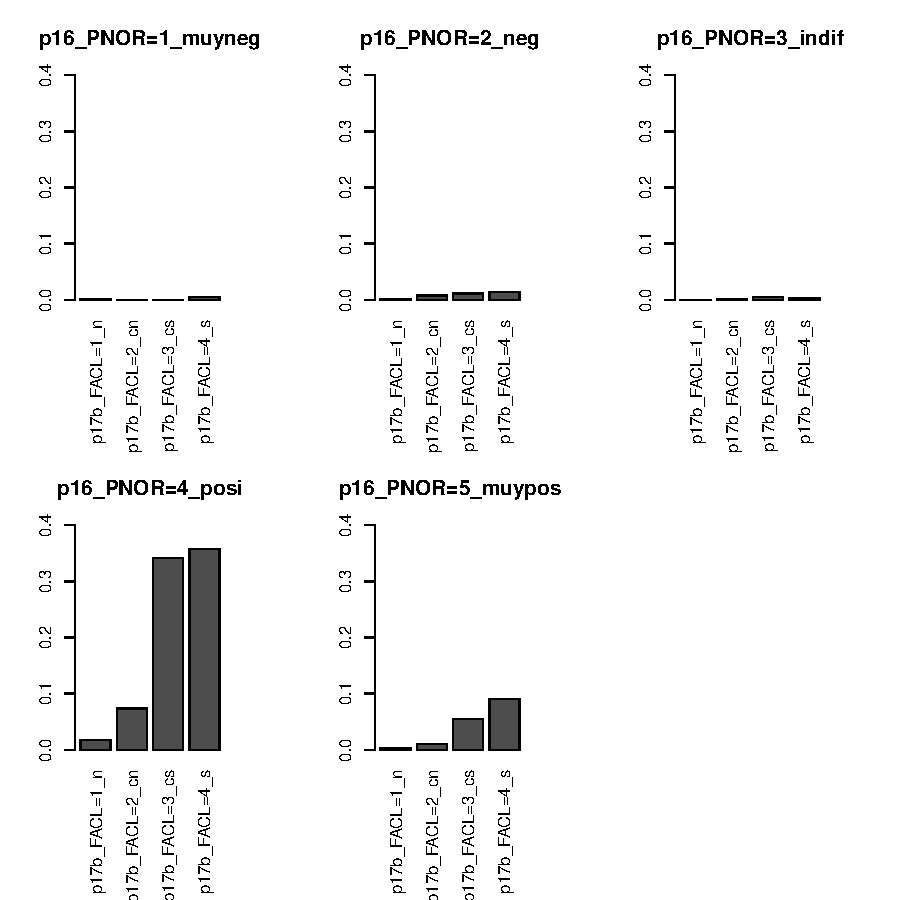
\includegraphics{5_ACS-barfrec}
	\caption{Frecuencias relativas}\label{fig:frecRelativas}
\end{figure}
\end{frame}

\begin{frame}
Una manera más eficiente de evitar los sesgos que producen los análisis directos sobre las frecuencias y las frecuencias relativas es utilizando las frecuencias relativas marginales, o condicionales también llamadas \textbf{perfiles} definidos como sigue:
\begin{align*}
	\text{Perfiles fila}\quad    & f_{i.} = \frac{n_{i.}}{n} = \frac1n \sum_{j=1}^{J} n_{ij} \\
	\text{Perfiles columna}\quad & f_{.j} = \frac{n_{.j}}{n} = \frac1n \sum_{i= 1}^{I} n_{ij}
\end{align*}
=> $f_{i.}$ es la frecuencia promedio de respuesta a la modalidad $i$ de la variable fila

=> $f_{.j}$ es la frecuencia promedio de respuesta a la modalidad $j$ de la variable columna
\end{frame}
% 
\begin{frame}
$$ \begin{array}{cccc|c}
f_{11}& f_{12}& \cdots& f_{1J} & f_{1.}\\
f_{21}& f_{22}& \cdots& f_{2J} & f_{2.}\\
\vdots& \vdots& \vdots& \vdots &  \\
f_{I1}& f_{I2}& \cdots& f_{IJ} & f_{I.}\\
\hline
f_{.1}& f_{.2}& \cdots& f_{.J} & 1
 \end{array},
 $$

=> la última columna contiene las frecuencias promedio de las modalidades de la variable fila

=> la última fila es el promedio de las frecuencias de las modalidades de la variable columna.

$G_{_I} = (f_{.1}, \ldots , f_{.J})$ centro de gravedad de filas (centroide)

$G_{_J} = (f_{1.}, \ldots , f_{I.})$  centro de gravedad columnas (centroide)

\end{frame}
% 



% 
\begin{frame}[fragile]
\begin{table}[!h]
\centering
\caption{\label{tab:perfilas}Tabla de perfiles fila para el sentimiento
      ante reglas o normas vs. facilidad para obedecer la ley}
\centering
\resizebox{\ifdim\width>\linewidth\linewidth\else\width\fi}{!}{
\begin{tabular}[t]{lrrrrr}
\toprule
  & p17b\_FACL=1\_n & p17b\_FACL=2\_cn & p17b\_FACL=3\_cs & p17b\_FACL=4\_s & TotFil\\
\midrule
\cellcolor{gray!10}{p16\_PNOR=1\_muyneg} & \cellcolor{gray!10}{0.12} & \cellcolor{gray!10}{0.00} & \cellcolor{gray!10}{0.00} & \cellcolor{gray!10}{0.88} & \cellcolor{gray!10}{1}\\
p16\_PNOR=2\_neg & 0.05 & 0.22 & 0.35 & 0.38 & 1\\
\cellcolor{gray!10}{p16\_PNOR=3\_indif} & \cellcolor{gray!10}{0.00} & \cellcolor{gray!10}{0.20} & \cellcolor{gray!10}{0.53} & \cellcolor{gray!10}{0.27} & \cellcolor{gray!10}{1}\\
p16\_PNOR=4\_posi & 0.02 & 0.09 & 0.43 & 0.45 & 1\\
\cellcolor{gray!10}{p16\_PNOR=5\_muypos} & \cellcolor{gray!10}{0.02} & \cellcolor{gray!10}{0.07} & \cellcolor{gray!10}{0.34} & \cellcolor{gray!10}{0.57} & \cellcolor{gray!10}{1}\\
\bottomrule
\end{tabular}}
\end{table}% 
\end{frame}

\begin{frame}
\setkeys{Gin}{width=2.8\textwidth, height=0.9\textheight,keepaspectratio} % para redefinir el tama?o de los graficos
\begin{figure}[H]
	\centering
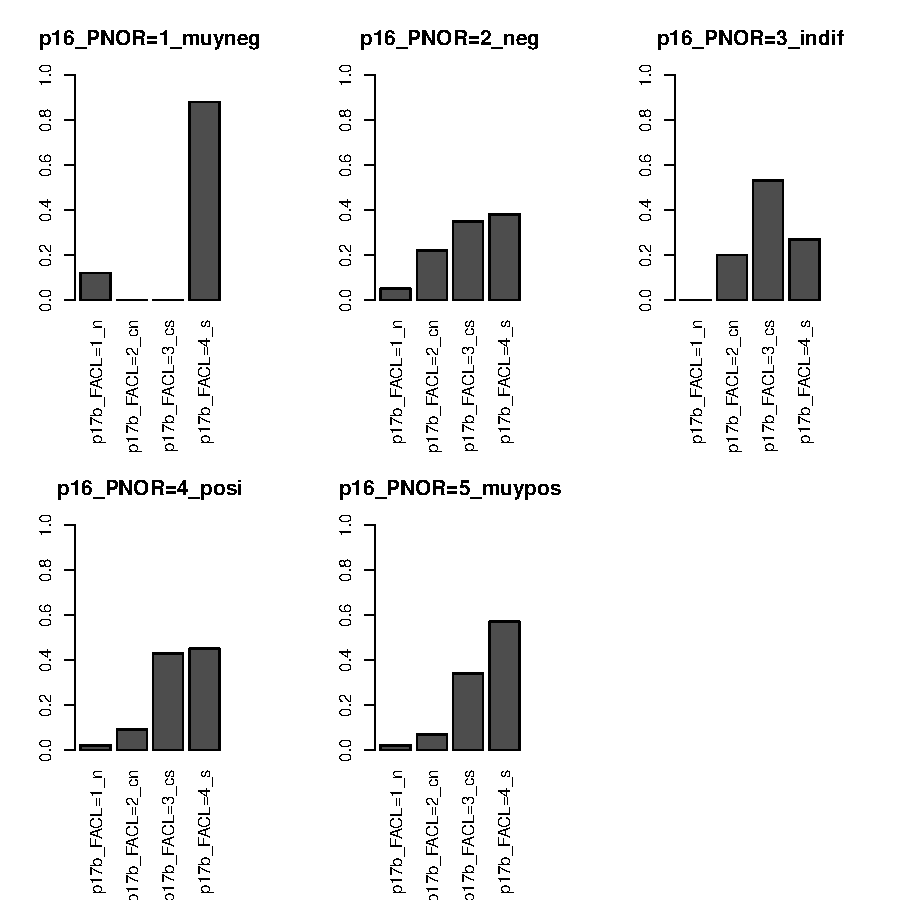
\includegraphics{5_ACS-barperfilas}
	\caption{Perfiles fila}\label{fig:perfilesfila}
\end{figure}
\end{frame}
% 
\begin{frame}
\begin{table}[!h]
\centering
\caption{\label{tab:percolumnas}Tabla de perfiles columna para el sentimiento
      ante reglas o normas vs. facilidad para obedecer la ley}
\centering
\resizebox{\ifdim\width>\linewidth\linewidth\else\width\fi}{!}{
\begin{tabular}[t]{lrrrr}
\toprule
  & p17b\_FACL=1\_n & p17b\_FACL=2\_cn & p17b\_FACL=3\_cs & p17b\_FACL=4\_s\\
\midrule
\cellcolor{gray!10}{p16\_PNOR=1\_muyneg} & \cellcolor{gray!10}{0.03} & \cellcolor{gray!10}{0.00} & \cellcolor{gray!10}{0.00} & \cellcolor{gray!10}{0.01}\\
p16\_PNOR=2\_neg & 0.08 & 0.08 & 0.03 & 0.03\\
\cellcolor{gray!10}{p16\_PNOR=3\_indif} & \cellcolor{gray!10}{0.00} & \cellcolor{gray!10}{0.02} & \cellcolor{gray!10}{0.01} & \cellcolor{gray!10}{0.01}\\
p16\_PNOR=4\_posi & 0.75 & 0.78 & 0.82 & 0.76\\
\cellcolor{gray!10}{p16\_PNOR=5\_muypos} & \cellcolor{gray!10}{0.14} & \cellcolor{gray!10}{0.12} & \cellcolor{gray!10}{0.13} & \cellcolor{gray!10}{0.19}\\
\addlinespace
Totcol & 1.00 & 1.00 & 1.00 & 1.00\\
\bottomrule
\end{tabular}}
\end{table}\end{frame}
% 
\begin{frame}
\setkeys{Gin}{width=3.2\textwidth, height=0.8\textheight,keepaspectratio} % para redefinir el tama?o de los graficos
\begin{figure}[H]
	\centering

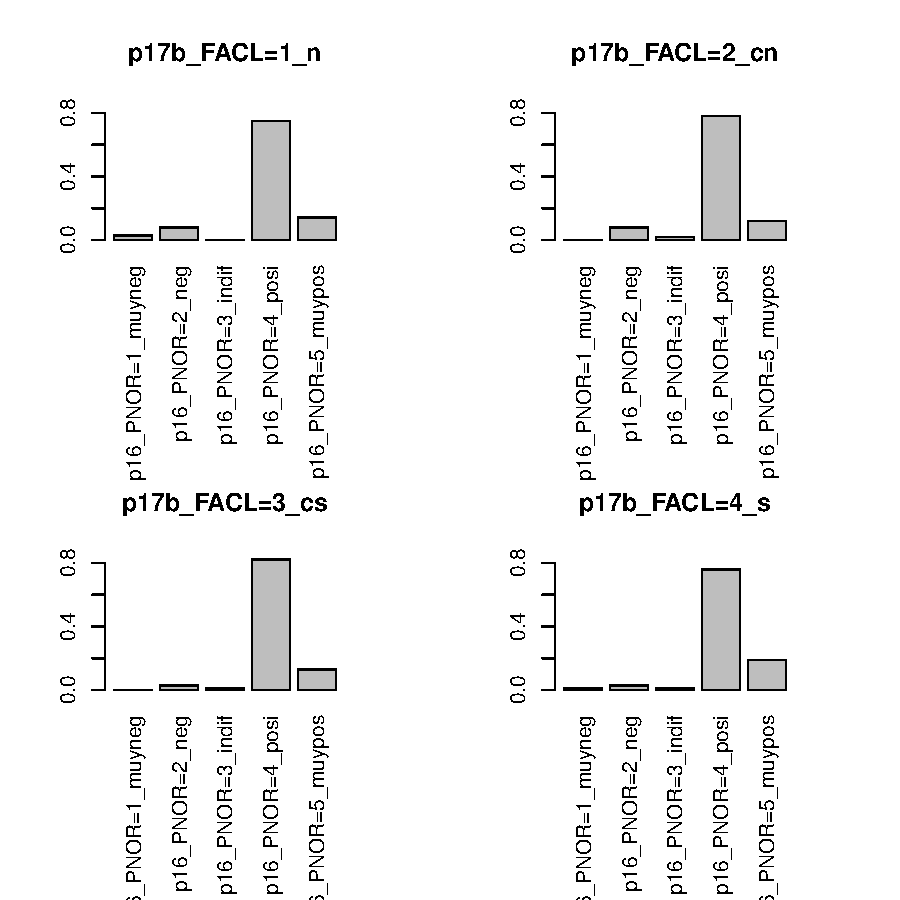
\includegraphics{5_ACS-barpercolumnas}
	\caption{Perfiles columna}\label{fig:perfilescol}
\end{figure}
\end{frame}
% 
\section{Obtención de los factores}
\begin{frame}{---------------\textcolor{yellow}{Obtención de los factores}---------------}
Por tratarse de una tabla de contingencia tanto el cálculo como la interpretación de los factores o componentes es un poco diferente al del ACP presentado en el capítulo anterior.

En las tablas de datos del ACP las filas representan objetos y las columnas son las variables, de manera que el análisis por filas es un análisis de similitudes entre objetos, el análisis por columnas es un análisis de correlación entre variables, mientras que el análisis simultáneo de filas y columnas indica la similitud de los objetos en términos de las variables observadas.
\end{frame}
% 
\begin{frame}
A diferencia del ACP, las tablas de datos para el ACS son tablas de contingencia en las cuales las filas y columnas representan las modalidades de dos variables cualitativas, y por tanto la interpretación de los dos análisis es la misma: 
por filas (columnas) se trata del análisis de asociación entre modalidades de la variable que está en las filas (columnas) y el análisis simultáneo de filas y columnas es para identificar el grado de asociación entre modalidades de las dos variables.
\end{frame}
% 
\begin{frame}
-- Adicionalmente, en ACP para el análisis de las columnas (variables) se utiliza la matriz de correlación, mientras que para el análisis de las filas (objetos) se utiliza la matriz de productos escalares entre éstos. 

-- Para el ACS en cambio, en lugar de una matriz de correlación no calculable con tablas de frecuencias, se utiliza una matriz de \textbf{distancias estandarizadas entre las frecuencias observadas y las frecuencias esperadas}. 
\end{frame}
% 
\begin{frame}
Las frecuencias esperadas se calculan bajo el supuesto de que las variables son independientes que se expresa en términos probabilísticos así: Sean $X$ la variable fila que tiene  $I$ modalidades y $Y$ la variable columna que tiene  $J$ modalidades. 

Entonces si las dos variables son independientes se cumple:
$$P(X=i,Y=j) = P(X=i)P(Y=j), \quad i=1,\ldots, I, \, j=1,\ldots, j  $$
\end{frame}
% 
\begin{frame}
\small
Empíricamente, si filas y columnas son independientes se espera que $f_{ij} = f_{i.}f_{.j} $ y por tanto se definen las \textbf{frecuencias esperadas} que corresponden las frecuencias que ocurrirían si las variables son independientes por:
\begin{align*}
& \hat{e}_{ij} = f_{i.}f_{.j}	
\end{align*}
Así las cosas, las diferencias entre las frecuencias observadas y las frecuencias esperadas  
$$f_{ij} - \hat{e}_{ij}$$
dan cuenta del grado de asociación entre las dos variables: 

-- si son pequeñas es porque las variables tienden a ser independientes

-- si son grandes indican cierto grado de asociación entre ellas. 
\end{frame}
% 
\begin{frame}
Entonces las distancias re-escaladas (estandarizadas) por las frecuencias esperadas se definen por:
\[
z_{ij} = \frac{f{ij} - \hat{e}_{ij}}{\sqrt{\hat{e}_{ij} } }
\]
de manera que si la distancia entre las frecuencias observadas y las esperadas es pequeña es porque las dos preguntas tienen modalidades independientes y por tanto no es necesario hacer ningún tipo de análisis.
\end{frame}
% 
\begin{frame}
La comparación entre frecuencias observadas y esperadas permite asociar el problema del análisis de asociación entre filas y columans de la tabla de contingencia con la estadística $\chi$ - cuadrado utilizada para probar la independencia como sigue. De la definición de la estadística $\chi^2$ se obtiene:
\begin{equation*}
	\chi^2=\sum_{i=1}^I\sum_{j=1}^J \frac{\left(n_{ij}- \frac{n_{i.}n_{.j}}{n}\right)^2}{\frac{n_{i.}n_{.j}}{n}}
	= n\sum_{i=1}^I\sum_{j=1}^J z_{ij}^2,
\end{equation*}
La segunda igualdad se consigue de multiplicar y dividir dentro del cuadrado por $n$.
\end{frame}
% 
\begin{frame}
En esta fórmula se evidencia que $\chi^2$ puede ser muy grande aún si las distancias entre lo observado y lo esperado no son muy grandes, dado que un $n$ suficientemente grande la hace crecer indefinidamente. Por esta razón, se define la inercia o dispersión para las distancias quitando el efecto del numero de observaciones por:
\begin{equation*}
	T=\frac{\chi^2}{n} = \sum_{i=1}^I\sum_{j=1}^J z_{ij}^2
\end{equation*}
\end{frame}
% 
\begin{frame}
En ACS las coordenadas para la representación de filas y columnas sobre el $\alpha$ - ésimo factor son combinaciones lineales (o sea promedios ponderados) de las distancias estandarizadas entre las frecuencias observadas y las esperadas:
\begin{align}
  r_{i\alpha} = \sum_{j=1}^{J}z_{ij}u_{j\alpha} = \sum_{j=1}^{J} \frac{f_{ij} - \hat{e}_{ij}}{\sqrt{\hat{e}_{ij} } }u_{j\alpha}   & \qquad \text{para las filas} \\
  c_{j\alpha} = \sum_{i=1}^{I}z_{ij}v_{i\alpha} = \sum_{i=1}^{I}\frac{f_{ij} - \hat{e}_{ij}}{\sqrt{\hat{e}_{ij} } }v_{i\alpha} & \qquad \text{para las columnas}
\end{align}
\end{frame}
% 
\begin{frame}
Un enfoque que produce los mismos resultados que el de las distancias $\chi^2$ consiste en proyectar directamente las frecuencias condicionales o perfiles de fila y columna definidos por:
\begin{align}
  \frac{f_{ij}}{f_{i.}} & \quad \quad \text{para las filas} & \frac{f_{ij}}{f_{.j}} & \quad \quad \text{para las columnas}
\end{align}

En este caso las coordenadas sobre el $\alpha$ - ésimo factor para las filas son:
\begin{equation*}
	r_{\alpha i}=\sum_{j=1}^J \frac{f_{ij}}{f_{i.}f_{.j}}u_{j\alpha}
	           =\frac{1}{f_{i.}} \sum_{j=1}^J \frac{f_{ij}}{f_{.j}}u_{j\alpha}
\end{equation*}
\end{frame}
% 
\begin{frame}{\textcolor{yellow}{-------------------Interpretación del ACS-------------------}}
\small
La principal diferencia grande con la interpretación del ACP es que en \textcolor{blue}{el ACS el análisis de filas y columnas es exactamente el mismo}, debido a que como tanto unas como otras representan las modalidades de respuesta de las dos variables analizadas. 

Por esta razón \textcolor{blue}{se hace un análisis por filas} o de puntos fila, \textcolor{blue}{un análisis por columnas} o de puntos columna y un \textcolor{blue}{análisis mixto de puntos fila y columna}. 

\textcolor{blue}{En el análisis por filas} (columnas), \textcolor{blue}{se identifican relaciones entre las modalidades de respuesta de la variable fila} (columna). 

El \textcolor{blue}{análisis mixto de puntos fila y columna} da cuenta de las \textcolor{blue}{relaciones entre las modalidades de las dos variables}.
\end{frame}
% 
\begin{frame}
 Los resultados se presentan también en planos factoriales acompañados de los porcentajes de varianza que aporta cada factor a la varianza total de las tablas. Las cercanías entre modalidades  (de filas o de columnas consideradas por separado), así como las cercanías entre modalidades mixtas de filas y columnas dan indicios de asociaciones entre ellas.
\end{frame}
% 
\begin{frame}{\textcolor{yellow}{-------------------Interpretación del ACS-------------------}}
\textbf{Coordenadas}
\small

\textbf{Puntos fila (columna), cercanos entre sí} indican grados de asociación entre las modalidades de respuesta de la variable que está en la filas (columnas). Puntos mixtos cercanos entre sí indican grados de asociación entre modalidades de las dos variables.
Modalidades de respuesta cercanas (fila, columna o mixtas) indican que las correspondientes modalidades fueron contestadas aproximadamente por los mismos individuos, o bien, que quienes las contestaron tienen opiniones son parecidas. Recíprocamente, modalidades alejadas indican bajas asociaciones entre modalidades y opiniones dispares entre quienes las contestaron.
\end{frame}
% 
\begin{frame}{\textcolor{yellow}{-------------------Interpretación del ACS-------------------}}
\textbf{Coordenadas}

\textbf{Puntos fila, columna, o mixtos, cercanos al centro del plano} indican frecuencias altas de respuesta a las modalidades que representan y por tanto se interpretan como puntos promedio (modales) de filas y columnas. Reflejan la opinión de la mayoría de los encuestados. Recíprocamente, puntos lejanos del centro del plano representan en general modalidades con bajas frecuencias de respuesta.
\end{frame}
% 
\begin{frame}{\textcolor{yellow}{-------------------Interpretación del ACS-------------------}}
\textbf{Coordenadas}

\textbf{Puntos fila, columna en extremos opuestos lejanos del origen del plano}, es decir, puntos que tienen coordenadas extemas con signos diferentes, no solo indicande bajas frecuencias de respuesta, sino que reflejan opiniones contrapuestas de quienes los contestaron.
\end{frame}
% 
\begin{frame}{\textcolor{yellow}{-------------------Interpretación del ACS-------------------}}
\small
\textbf{Contribuciones:} aportes de las modalidades a la varianza del factor. 

$r_{\alpha i}$ la coordenada de la modalidad $i$ sobre el $\alpha$ - ésimo factor de la pregunta $p_1$,

$r_{\alpha j}$  la coordenada de la modalidad $j$ de la pregunta $p_2$

las contribuciones de las modalidades son las proporciones de varianza $\lambda_{\alpha}$ del factor ponderadas por la proporción de respuestas a la modalidad $f_{i.}$ definidas por:
		\begin{gather}
\text{\textbf{contribución de la modalidad} $i$ de $p_1$}\quad	C_\alpha(i)=\frac{f_{i.}r_{\alpha i}^2}{\lambda_{\alpha}}\notag \\
\text{\textbf{contribución de la modalidad} $j$ de la  $p_2$}\quad		C_\alpha(j)=\frac{f_{.j}r_{\alpha j}^2}{\lambda_{\alpha}}
	\end{gather}
Modalidades con coordenadas y contribuciones altas se utilizan para tipificarlo y eventualmente utilizarlo como indicador de las propiedades definidas por dichas modalidades.
\end{frame}
% 
\begin{frame}{\textcolor{yellow}{-------------------Interpretación del ACS-------------------}}
\small
\textbf{Cosenos cuadrados:} Indican el grado de representación de una modalidad sobre el factor. 

Dan cuenta de la capacidad del factor para predecir o representar la modalidad.
Sean $d^2(i,G)$ y $d^2(j,G)$ las distancias de la modalidad $i$ de $p_1$ y $j$ de $p_2$ a sus centros de gravedad $G_{_I} = (f_{.1}, \ldots , f_{.J})$ y $G_{_J} = (f_{1.}, \ldots , f_{I.})$  respectivamente.
Entonces los cosenos cuadrados se calculan como sigue:
		\begin{gather}
\text{aporte del $\alpha$-ésimo factor a la modalidad $i$ de $p_1$}\quad cos^2_\alpha(i)=\frac{r^2_{\alpha i}}{d^2(i,G_{_I})}\notag \\
\text{aporte del $\alpha$-ésimo factor a la modalidad $j$ de $p_2$}\quad cos^2_\alpha(i)=\frac{r^2_{\alpha j}}{d^2(j,G_{_J})}
    \end{gather}
Entre más cercano a uno sea el coseno cuadrado, mejor representada está la modalidad sobre el factor y por tanto es un buen representante de ésta.
\end{frame}
% 
\begin{frame}{\textcolor{yellow}{-------------------Interpretación del ACS-------------------}}
\textbf{Modalidades poco frecuentes}

Una de las propiedades del ACS es que aleja del origen del plano las modalidades poco frecuentes, identificando así las características que más distinguen a los objetos. Y como complemento aquellas moddalidades con frecuencias altas quedan representadas en el centro.
\end{frame}
% 
\section{Ejemplos}
\begin{frame}[fragile]
{Ejemplo: Encuesta de Cultura Ciudadana}
Para corroborar la conjetura acerca de la relación entre las modalidades de respuesta de las preguntas p16 sobre la facilidad para cumplir la ley, y p17b acerca de los sentimientos ante palabras como regla o norma de la ECC del ejemplo \ref{ECC1} según la cual sentimientos positivos hacia las reglas o normas deberían ir asociados con la facilidad para cumplirlas, se lleva a cabo un ACS de la Tabla \ref{tab:pr16x17} y se proyectan las respuestas sobre los dos primeros factores en la gráfica \ref{fig:PlanoincumAcuerd}

\end{frame}
% 
\begin{frame}[fragile]
{\textcolor{yellow}{Análisis por filas}}
\scriptsize 
\begin{table}[!h]
\centering
\caption{\label{tab:InParaInterprertar}Coordenadas, contribuciones y cosenos cuadrados}
\centering
\begin{tabular}[t]{lrrrrrr}
\toprule
\multicolumn{1}{c}{ } & \multicolumn{2}{c}{Coord} & \multicolumn{2}{c}{Contr} & \multicolumn{2}{c}{Cos2} \\
\cmidrule(l{3pt}r{3pt}){2-3} \cmidrule(l{3pt}r{3pt}){4-5} \cmidrule(l{3pt}r{3pt}){6-7}
  & Factor 1 & Factor 2 & Factor 1 & Factor 2 & Factor 1 & Factor 2\\
\midrule
\cellcolor{gray!10}{p16\_PNOR=1\_muyneg} & \cellcolor{gray!10}{-0.94} & \cellcolor{gray!10}{0.60} & \cellcolor{gray!10}{28.84} & \cellcolor{gray!10}{22.46} & \cellcolor{gray!10}{0.68} & \cellcolor{gray!10}{0.28}\\
p16\_PNOR=2\_neg & 0.25 & 0.41 & 13.91 & 72.25 & 0.27 & 0.73\\
\cellcolor{gray!10}{p16\_PNOR=3\_indif} & \cellcolor{gray!10}{0.50} & \cellcolor{gray!10}{-0.01} & \cellcolor{gray!10}{15.21} & \cellcolor{gray!10}{0.01} & \cellcolor{gray!10}{0.94} & \cellcolor{gray!10}{0.00}\\
p16\_PNOR=4\_posi & 0.03 & -0.02 & 3.96 & 5.24 & 0.52 & 0.36\\
\cellcolor{gray!10}{p16\_PNOR=5\_muypos} & \cellcolor{gray!10}{-0.19} & \cellcolor{gray!10}{0.01} & \cellcolor{gray!10}{38.09} & \cellcolor{gray!10}{0.05} & \cellcolor{gray!10}{0.92} & \cellcolor{gray!10}{0.00}\\
\bottomrule
\end{tabular}
\end{table}
\end{frame}
% 
\begin{frame}[fragile]
{\textcolor{yellow}{Análisis por filas}}
\setkeys{Gin}{width=0.6\textwidth} % redefinir el tama?o graficos
\begin{figure}[H]
	\centering
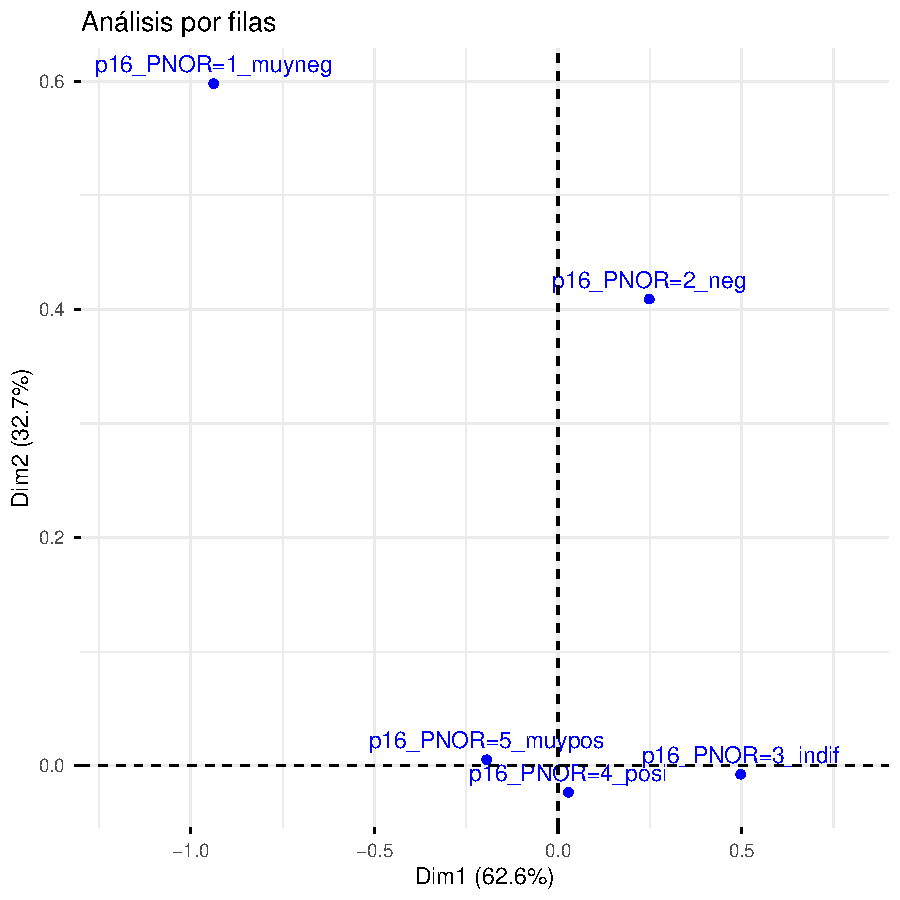
\includegraphics{5_ACS-024}
	\caption{Análisis por filas: Sentimientos ante palabras como regla o norma. Sobresalen lejos del origen, las dos modalidades con más bajas frecuencias sobre el Factor 2.}\label{fig:P1_2_SentiReglas}
\end{figure}

\end{frame}
% 
\begin{frame}[fragile]
{\textcolor{yellow}{Análisis por columnas}}
\scriptsize
\begin{table}[!h]
\centering
\caption{\label{tab:Interprertarcols}Coordenadas, contribuciones y cosenos cuadrados}
\centering
\begin{tabular}[t]{lrrrrrr}
\toprule
\multicolumn{1}{c}{ } & \multicolumn{2}{c}{Coord} & \multicolumn{2}{c}{Contr} & \multicolumn{2}{c}{Cos2} \\
\cmidrule(l{3pt}r{3pt}){2-3} \cmidrule(l{3pt}r{3pt}){4-5} \cmidrule(l{3pt}r{3pt}){6-7}
  & Factor 1 & Factor 2 & Factor 1 & Factor 2 & Factor 1 & Factor 2\\
\midrule
\cellcolor{gray!10}{p17b\_FACL=1\_n} & \cellcolor{gray!10}{-0.09} & \cellcolor{gray!10}{0.37} & \cellcolor{gray!10}{1.15} & \cellcolor{gray!10}{38.85} & \cellcolor{gray!10}{0.04} & \cellcolor{gray!10}{0.79}\\
p17b\_FACL=2\_cn & 0.24 & 0.18 & 33.81 & 35.04 & 0.63 & 0.34\\
\cellcolor{gray!10}{p17b\_FACL=3\_cs} & \cellcolor{gray!10}{0.09} & \cellcolor{gray!10}{-0.07} & \cellcolor{gray!10}{20.79} & \cellcolor{gray!10}{25.62} & \cellcolor{gray!10}{0.59} & \cellcolor{gray!10}{0.38}\\
p17b\_FACL=4\_s & -0.12 & 0.01 & 44.25 & 0.49 & 0.98 & 0.01\\
\bottomrule
\end{tabular}
\end{table}
\end{frame}
% 
\begin{frame}[fragile]
{\textcolor{yellow}{Análisis por columnas}}

\setkeys{Gin}{width=0.6\textwidth} % redefinir el tama?o graficos
\begin{figure}[H]
	\centering
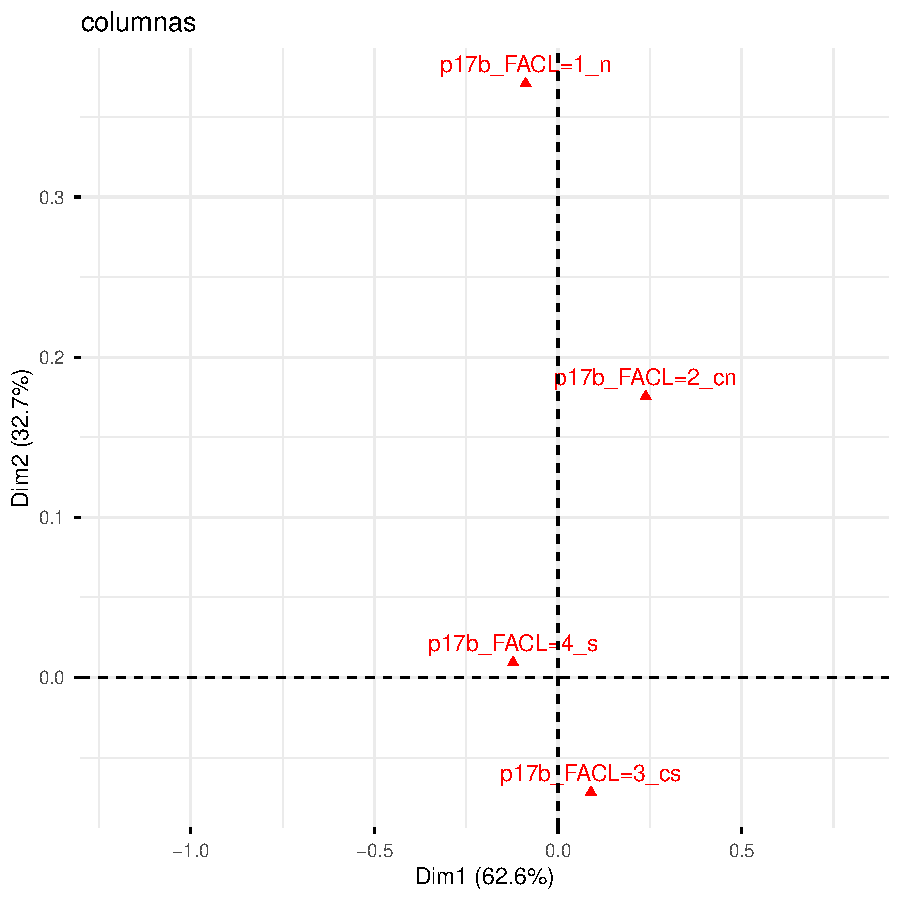
\includegraphics{5_ACS-026}
	\caption{Faciliadad para actuar conforme a la ley. Sobresalen lejos del origen las modalidades nunca y casi nunca, modalidades con bajas frecuencias que son las que más distinguen a los encuestados.}\label{fig:PlanoFacilLye}
\end{figure}
\end{frame}
%
% 
\begin{frame}[fragile]
{\textcolor{yellow}{Representación simultánea: }}
{Relaciones entre filas y columnas}
\setkeys{Gin}{width=3.5\textwidth, height=0.8\textheight,keepaspectratio} % para redefinir el tama?o de los
\begin{figure}[H]
	\centering
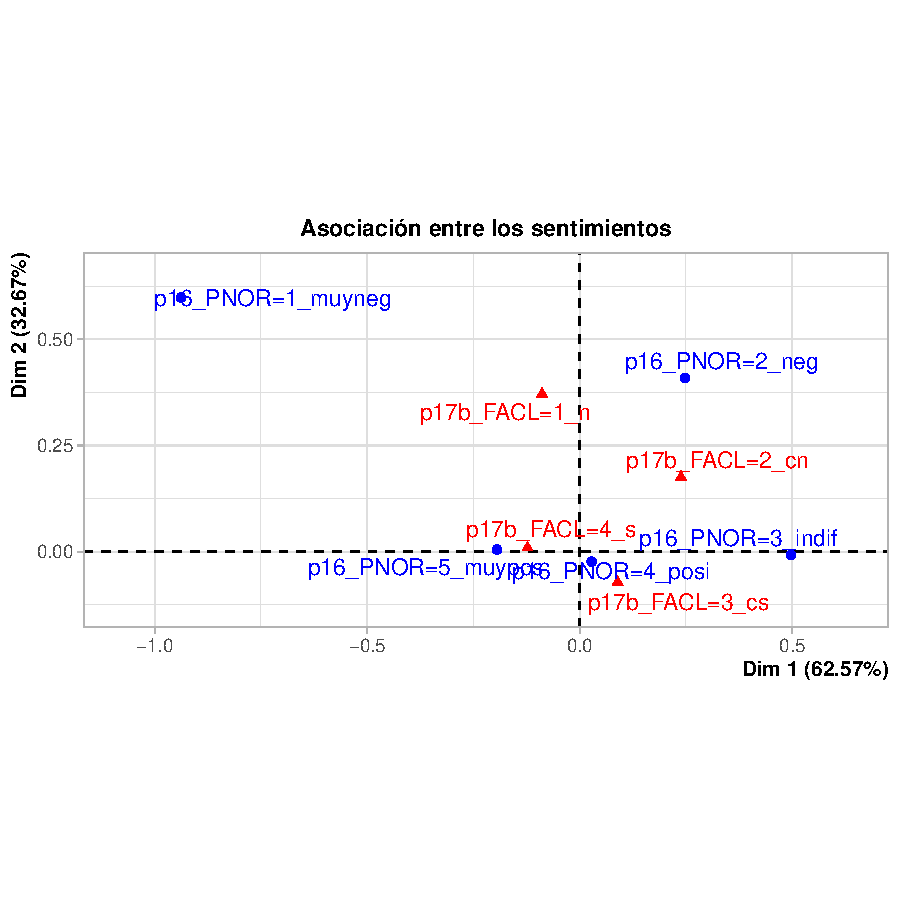
\includegraphics{5_ACS-029}
	\caption{Sentimientos ante palabras como regla o norma y facilidad para actuar conforme a la ley.}\label{fig:PlanoincumAcuerd}
\end{figure}
\end{frame}
% 
\begin{frame}{Referncias de interés}
\bibliography{BiblioMultivariado}
\end{frame}
% 
% \begin{frame}
% 
% \end{frame}
% 
% \begin{frame}
% 
% \end{frame}
% 
% \begin{frame}
% 
% \end{frame}
% 
% \begin{frame}
% 
% \end{frame}
% 
% \begin{frame}
% 
% \end{frame}
% 
% \begin{frame}
% 
% \end{frame}
% 
% \begin{frame}
% 
% \end{frame}
% 
% \begin{frame}
% 
% \end{frame}


\end{document}


